\chapter[Basics of SCUFF-EM Software][Basics of SCUFF-EM Software]{Basics of SCUFF-EM Software} \label{ap:SCUFFEM}

\section{Introduction}
%
In this appendix, instructions are provided to perform NFRHT simulations using \textsc{scuff-em}, which is short for Surface CUrrent/Field Formulation of ElectroMagnetism. \textsc{scuff-em} is a free, open-source software implementation of the boundary-element method \cite{scuffem, Reid2015} which models fluctuating-surface-currents as the source of thermal radiation. The source code for \textsc{scuff-em} is available at \url{https://github.com/HomerReid/scuff-em/}.

Instructions will be provided assuming installation on a computer running Ubuntu 14.04 locally. Some modification may be required when using other systems. These instructions are meant to be supplemental to the existing \href{http://homerreid.github.io/scuff-em-documentation/}{\textsc{scuff-em} documentation} and will not cover all features of the software. They will, however, cover all steps required to perform the NFRHT calculations completed in this dissertation. Broadly speaking, there are three main steps: (1) Create and mesh each object. (2) Define the configuration of all objects. (3) Feed the appropriate files to \textsc{scuff-em} to run a simulation. These steps are described below.


\section{Creating the Mesh}
%
\textsc{scuff-em} requires meshed surfaces, and the free software \href{http://gmsh.info/}{Gmsh} is recommended to create the meshes. The first step is to create a Gmsh geometry file for each unique object. For a sphere, such a file looks like Listing \ref{lst:GmshGeometry}. The value of $R$ given in line 8 should be given in micrometers. The meshing finenesses given in lines 13-15 should be adjusted depending on the geometry being investigated. For a uniform mesh, set $l1=l2=l3$. In this appendix, I will show an example for NFRHT between two spheres. In that situation, it is advantageous for increase the density of the mesh at a single pole only, in this case the north pole. The point, circle, line loop, ruled surface, and physical surface commands on lines 20-55 are used to build a boundary representation of a sphere from primitive objects like points and arcs. For further information, I direct readers to the \href{http://gmsh.info/doc/texinfo/gmsh.html}{Gmsh documentation}. The file given in Listing \ref{lst:GmshGeometry} may be used for any sphere by altering the values on lines 8, 13, 14, and 15.

\singlespacing
\begin{lstlisting}[language=C++, caption={Gmsh geometry file for a sphere.}, label={lst:GmshGeometry}]
//
// Gmsh geometry specification for a sphere of radius R
// 

//************************************************************
//* input parameters      
//************************************************************
R = 10.0;    // radius

//************************************************************
//* meshing finenesses ***************************************
//************************************************************
l3 = 0.10;  // fineness at north pole
l2 = 1.00;  // fineness at equator
l1 = 1.00;  // fineness at south pole

//************************************************************
//* defintion of sphere *********************************************
//************************************************************
Point(1) = {  0 ,    0,  0.0,  l2};
Point(2) = {  R,    0,  0.0,  l2};
Point(3) = {  0 ,   R,  0.0,  l2};
Circle(1) = {2,1,3};
Point(4) = { -R,    0,  0.0,  l2};
Point(5) = {   0,  -R,  0.0,  l2};
Circle(2) = {3,1,4};
Circle(3) = {4,1,5};
Circle(4) = {5,1,2};
Point(6) = {   0,    0,  0.0+R, l3};
Point(7) = {   0,    0,  0.0-R, l1};
Circle(5) = {3,1,6};
Circle(6) = {6,1,5};
Circle(7) = {5,1,7};
Circle(8) = {7,1,3};
Circle(9) = {2,1,7};
Circle(10) = {7,1,4};
Circle(11) = {4,1,6};
Circle(12) = {6,1,2};
Line Loop(13) = {2,8,-10};
Ruled Surface(14) = {13};
Line Loop(15) = {10,3,7};
Ruled Surface(16) = {15};
Line Loop(17) = {-8,-9,1};
Ruled Surface(18) = {17};
Line Loop(19) = {-11,-2,5};
Ruled Surface(20) = {19};
Line Loop(21) = {-5,-12,-1};
Ruled Surface(22) = {21};
Line Loop(23) = {-3,11,6};
Ruled Surface(24) = {23};
Line Loop(25) = {-7,4,9};
Ruled Surface(26) = {25};
Line Loop(27) = {-4,12,-6};
Ruled Surface(28) = {27};
Physical Surface(1) = {28,26,16,14,20,24,22,18};

//************************************************************
//* reference point to get outward-pointing surface normals right
//************************************************************
Physical Point(1) = {1};
\end{lstlisting}
\doublespacing

Next, Gmsh must be used to generate a mesh file from the geometry file. This can be done through the terminal window. If the geometry file given in Listing \ref{lst:GmshGeometry} is saved as Geometry.geo in the current working directory, a mesh file, called Mesh.msh, is generated by the command
%
\begin{lstlisting}[language=C++]
gmsh -2 -clscale 5.0 Geometry.geo -format msh2 -o Mesh.msh
\end{lstlisting}
%
where the -clscale parameter controls the fineness of the mesh. Its value can be decreased to create a finer mesh, or increased to create a less dense mesh. The same mesh may be used for two identical objects; separate mesh files must be generated for any unique objects.  


\section{Defining the Configuration}
%
Now that the mesh file has been created, the \textsc{scuff-em} geometry file is next. \textsc{scuff-em} geometry files carry the extension .scuffgeo and define the orientation, location, mesh file, and optical properties of each object. An example of a \textsc{scuff-em} geometry file is given in Listing \ref{lst:SCUFFGeometry} for two silicon dioxide spheres separated by a center-to-center distance of 15 \si{\micro\meter}.

\singlespacing
\begin{lstlisting}[language=Perl, caption={\textsc{scuff-em} geometry file.}, label={lst:SCUFFGeometry}]
# dielectric model for silicon dioxide
MATERIAL SIO2
	A1 = 8.2736e+13;
 	w01 = 8.54484e+13;
 	G1 = 8.46448e+12;
 	A2 = 1.58004e+14;
 	w02 = 2.029e+14;
 	G2 = 1.06449e+13;
 	A3 = 3.39786e+13;
 	w03 = 1.51198e+14;
 	G3 = 8.33205e+12;
 	EpsInf = 2.03843;
 
 	Eps(w) = EpsInf + A1*A1/(w01*w01 - w*w - i*w*G1) + A2*A2/(w02*w02 - w*w - i*w*G2) + A3*A3/(w03*w03 - w*w - i*w*G3);
ENDMATERIAL

OBJECT Sphere1
	MESHFILE Mesh.msh
	MATERIAL SIO2
ENDOBJECT

OBJECT Sphere2
	MESHFILE Mesh.msh
	MATERIAL SIO2
	ROTATED 180 ABOUT 1 0 0
	DISPLACED 0 0 25.0
ENDOBJECT
\end{lstlisting}
\doublespacing

There are two main components to the \textsc{scuff-em} geometry file: material declarations and object declarations. Material declarations provide the dielectric function of a given material and should appear first in a \textsc{scuff-em} geometry file. Multiple materials may be defined sequentially. Advanced users may also choose to locate their material declarations in a central repository. \textsc{scuff-em} has two built-in materials: vacuum and perfect electrical conductor (PEC). The dielectric function must be calculated in units of $u = \omega/\omega_{0}$ where $\omega_{0} = 3 \times 10^{14}$ \si{\radian\per\second}. To convert from wavelength $\lambda$ (in micrometers) to $u$, use $\lambda = 2\pi/u$

Object declarations are used for finite objects, bounded by finite surfaces, which are not touching any other objects. They specify the mesh file, material, and configuration using the MESHFILE, MATERIAL, and ROTATED/DISPLACED keywords, respectively. MESHFILE refers to a previously created mesh, which should be stored in the current working directory or in a central repository. MATERIAL refers to the previously discussed material declaration. Failure to provide MATERIAL results in an object being treated as a PEC. ROTATED refers to the orientation of the object's intrinsic coordinate axes relative to the global axes. ROTATED has arguments $d$ ABOUT $ax$ $ay$ $az$, where $d$ is the rotation (in degrees) and $ax$, $ay$, $az$ correspond to the $x$, $y$, and $z$-axes. The ROTATED command in Listing \ref{lst:SCUFFGeometry} produces a rotation about the $x$-axis of 180 degrees. DISPLACED refers to the Cartesian translation of an object's intrinsic origin relative to the global coordinate system's origin. For the sphere defined above, the intrinsic origin lies at the sphere's center. Failure to provide values for DISPLACED results in the object's axes and origin to be aligned with a global set of axes and a global origin. The DISPLACED keyword takes three arguments: $x$ $y$ $z$. For example in Listing \ref{lst:SCUFFGeometry}, Sphere2 is translated 25 \si{\micro\meter} in the positive z-direction. Since Sphere1 and Sphere2 have radii of 10 \si{\micro\meter}, they are separated by a minimum separation distance of 5 \si{\micro\meter}. The ROTATED and DISPLACED commands are read sequentially, so care must be taken to ensure they are given in the intended order. For example, if lines 25 (ROTATED) and 26 (DISPLACED) are reversed in Listing \ref{lst:SCUFFGeometry}, the translation and rotation of Sphere2 will result in its origin being located at $(0,0,-25)$ instead of $(0,0,25)$. 

It is important to note that there are many other more advanced features which may be included in a \textsc{scuff-em} geometry file. I direct readers to \url{http://homerreid.github.io/scuff-em-documentation/reference/Geometries/} for further details.

Once a \textsc{scuff-em} geometry file is created, I advise visually checking the resulting geometry using Gmsh. To do so, use the terminal command
%
\begin{lstlisting}[language=C++]
scuff-analyze --geometry Geometry.scuffgeo --WriteGMSHFiles
\end{lstlisting}
%
and then open the resulting file with the extension .pp using Gmsh. For the example presented above, the result is shown in Fig. \ref{fig:SCUFF_Visualization}. The bottom sphere is Sphere1 and the top sphere is Sphere2. Sphere1 clearly shows the denser mesh at its northern pole; the underside of Sphere2 is identical.

\begin{figure}
\centering
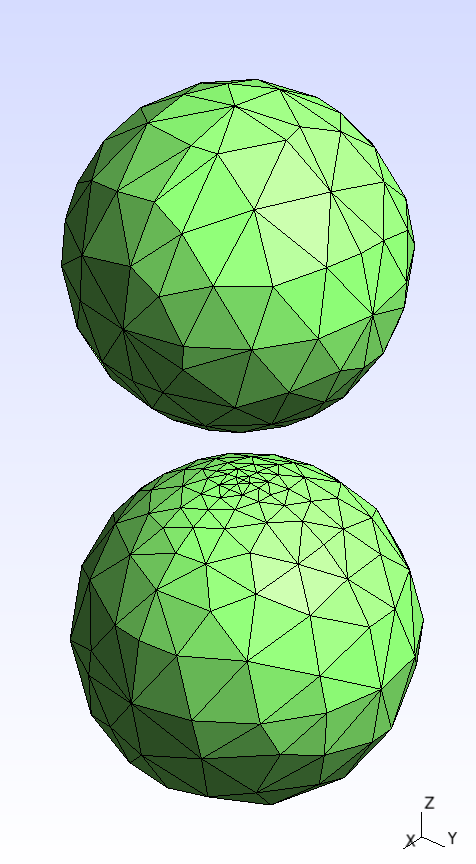
\includegraphics[width=0.35\textwidth]{./Figures/SCUFF_Visualization.png}
\caption{\label{fig:SCUFF_Visualization}Visualization of the \textsc{scuff-em} geometry file, created using Gmsh.}
\end{figure}


\section{Running a Simulation}
%
To run a single NFRHT simulation, we will call upon the code for non-equilibrium (NEQ) fluctuation-induced phenomena. It can handle both NFRHT and Casimir force calculations. We are interested in calculating the transmissivity function between objects. In the parlance of SCUFF-EM, it is called the generalized flux, $\Phi_{s \rightarrow d}(u)$. The generalized flux output by SCUFF-EM is exactly equal to $\tau_{s \rightarrow d}(\omega)$ from Eq. \ref{eq:NetHeatTransfer}. The command to compute NFRHT is
%
\begin{lstlisting}[language=C++]
scuff-neq --geometry Geometry.scuffgeo --OmegaFile OmegaFile
\end{lstlisting}
%
where OmegaFile is a file of values of $u$ at which $\Phi_{s \rightarrow d}(u)$ will be evaluated. Each value of $u$ in OmegaFile should occupy its own line. The example showed is the most basic NFRHT calculation. Several customizations are available, and I direct readers to \url{http://homerreid.github.io/scuff-em-documentation/applications/scuff-neq/scuff-neq/} for all of them.

There is one special option to which I will draw attention: transformations. Many elements of the scattering matrix used to compute NFRHT require properties of the individual bodies alone, and thus can be reused if a heat transfer-distance is desired. In order to save computational time, a transformation file can be supplied which details all the translations (or rotations) desired. The transformation file should give all translations and rotations relative to the configuration given in the \textsc{scuff-em} geometry file. For example, a file which takes our spheres and also computes NFRHT with minimum separation gaps of 10, 15, and 20 \si{\micro\meter} would read

\singlespacing
\begin{lstlisting}[language=Perl, caption={\textsc{scuff-em} transformation file.}, label={lst:SCUFFTransformation}]
TRANS 5  OBJECT Sphere2 DISP 0 0  0
TRANS 10 OBJECT Sphere2 DISP 0 0  5
TRANS 15 OBJECT Sphere2 DISP 0 0  10
TRANS 20 OBJECT Sphere2 DISP 0 0  15
\end{lstlisting}
\doublespacing
%
where the second column is a label, the fourth column is the object being transformed, and the sixth, seventh, and eighth columns are the Cartesian translations (relative to the \textsc{scuff-em} geometry file). There are a number of more sophisticated transformation methods allowed, which are covered extensively in \url{http://homerreid.github.io/scuff-em-documentation/reference/Transformations/}. The command to execute a NFRHT simulation using a transformation file is

\singlespacing
\begin{lstlisting}[language=C++]
scuff-neq --geometry Geometry.scuffgeo --TransFile Transformation --OmegaFile OmegaFile
\end{lstlisting}
\doublespacing
%
where Transformation is the \textsc{scuff-em} transformation file.

The result of such a command is a file called Geometry.SIFlux.EMTPFT where SI refers to the result being spatially integrated and EMTPFT (energy-momentum transfer, power force torque) refers to the method of integration (EMTPFT is the default method). An example output file is given in Listing \ref{lst:SCUFFExampleResults} for two objects and two frequencies. The columns of the file are the (1) transformation label (0.0 if no transformation file is provided), (2) non-dimensional frequency $u$, (3) source and destination objects, (4) flux spectral density of absorbed power ($\Phi_{s \rightarrow d}$), (5) flux spectral density of radiated power, (6-8) $x$, $y$, and $z$ components of force flux spectral density, and (9-11) $x$, $y$, and $z$ components of torque flux spectral density.

\singlespacing
\begin{lstlisting}[language=Perl, caption=Sample output file from {\textsc{scuff-em}.}, label={lst:SCUFFExampleResults}]
# scuff-neq run on Lab127 (08/29/18::18:33:30)
# data file columns: 
# 1 transform tag
# 2 omega 
# 3 (sourceSurface,destSurface) 
# 4 PAbs flux spectral density
# 5 PRad flux spectral density
# 6 XForce flux spectral density
# 7 YForce flux spectral density
# 8 ZForce flux spectral density
# 9 XTorque flux spectral density
# 10 YTorque flux spectral density
# 11 ZTorque flux spectral density
0.0 1.256637e+00 11 -7.90281126e-03 +7.90281126e-03 +2.69890579e-09 +8.84873807e-09 +5.63661446e-06 +3.61864629e-07 -3.84970743e-07 +1.83454544e-07 
0.0 1.256637e+00 12 +3.13534531e-07 -3.13534531e-07 -2.31817174e-10 -8.73833724e-10 +3.15096081e-06 +7.15556954e-09 -1.58668386e-07 +3.72063847e-09 
0.0 1.256637e+00 21 +3.13534530e-07 -3.13534530e-07 +3.49548060e-10 +8.71691790e-10 -3.15110593e-06 -8.50545313e-09 -1.70369659e-08 +1.50823996e-09 
0.0 1.256637e+00 22 -7.90281156e-03 +7.90281156e-03 +3.03177834e-09 +8.33691980e-09 -5.65780382e-06 -8.43395835e-05 +3.44041141e-05 +1.84850281e-07 
0.0 1.231997e+00 11 -8.12161225e-03 +8.12161225e-03 +2.33929940e-09 +8.21665833e-09 -1.23062421e-06 +3.92032030e-07 -4.11282818e-07 +1.79000346e-07 
0.0 1.231997e+00 12 +3.44786515e-07 -3.44786515e-07 -2.21137091e-10 -8.30112384e-10 +2.79435617e-06 +4.43090059e-09 -1.52735690e-07 +3.57295128e-09 
0.0 1.231997e+00 21 +3.44786514e-07 -3.44786514e-07 +3.41479370e-10 +8.37460786e-10 -2.79450235e-06 +4.12857975e-09 -2.13249109e-08 -6.37395124e-10 
0.0 1.231997e+00 22 -8.12161250e-03 +8.12161250e-03 +2.99997828e-09 +7.74714497e-09 +1.21073213e-06 -8.33215031e-05 +3.39882913e-05 +1.82055594e-07
\end{lstlisting}
\doublespacing
%

For NFRHT calculations, columns 6 through 11 may be ignored. $\tau_{s \rightarrow d}(\omega)$, defined in Eq. \ref{eq:NetHeatTransfer}, is exactly equal to the value of $\Phi_{s \rightarrow d}(u)$ located in column 4 for $s \ne d$. $\tau_{s \rightarrow E}(\omega)$, the transmissivity function defined between an object and its environment, is not given directly by \textsc{SCUFF-EM}. Instead, it must be obtained using quantities from column 4 and 
\begin{equation}
\tau_{s \rightarrow E}(\omega) = -\sum_{\alpha} \Phi_{s \rightarrow \alpha}
\end{equation}
%
where $\alpha$ is an index over all objects, including $\alpha=s$. The self-contribution to the transmissivity is negative and has a large magnitude, so $\tau_{s \rightarrow E} > 0$. For an isolated object, $\tau_{s \rightarrow E} = \Phi_{s \rightarrow s}$.